%-------------------------------------------------------------------------
% q-info-S1-preambule.tex
%-------------------------------------------------------------------------


\mbox{}\hfill
\begin{minipage}{9cm}\footnotesize
\textbf{Questionnement}, subst. masc., Fait de poser un ensemble 
de questions sur un problème.\\
\mbox{}\hfill Centre national de ressources textuelles et lexicales (\href{http://www.cnrtl.fr/definition/questionnement}{\textsc{Cnrtl}})
\end{minipage}
\vspace*{5mm}

%\newpage
%\noindent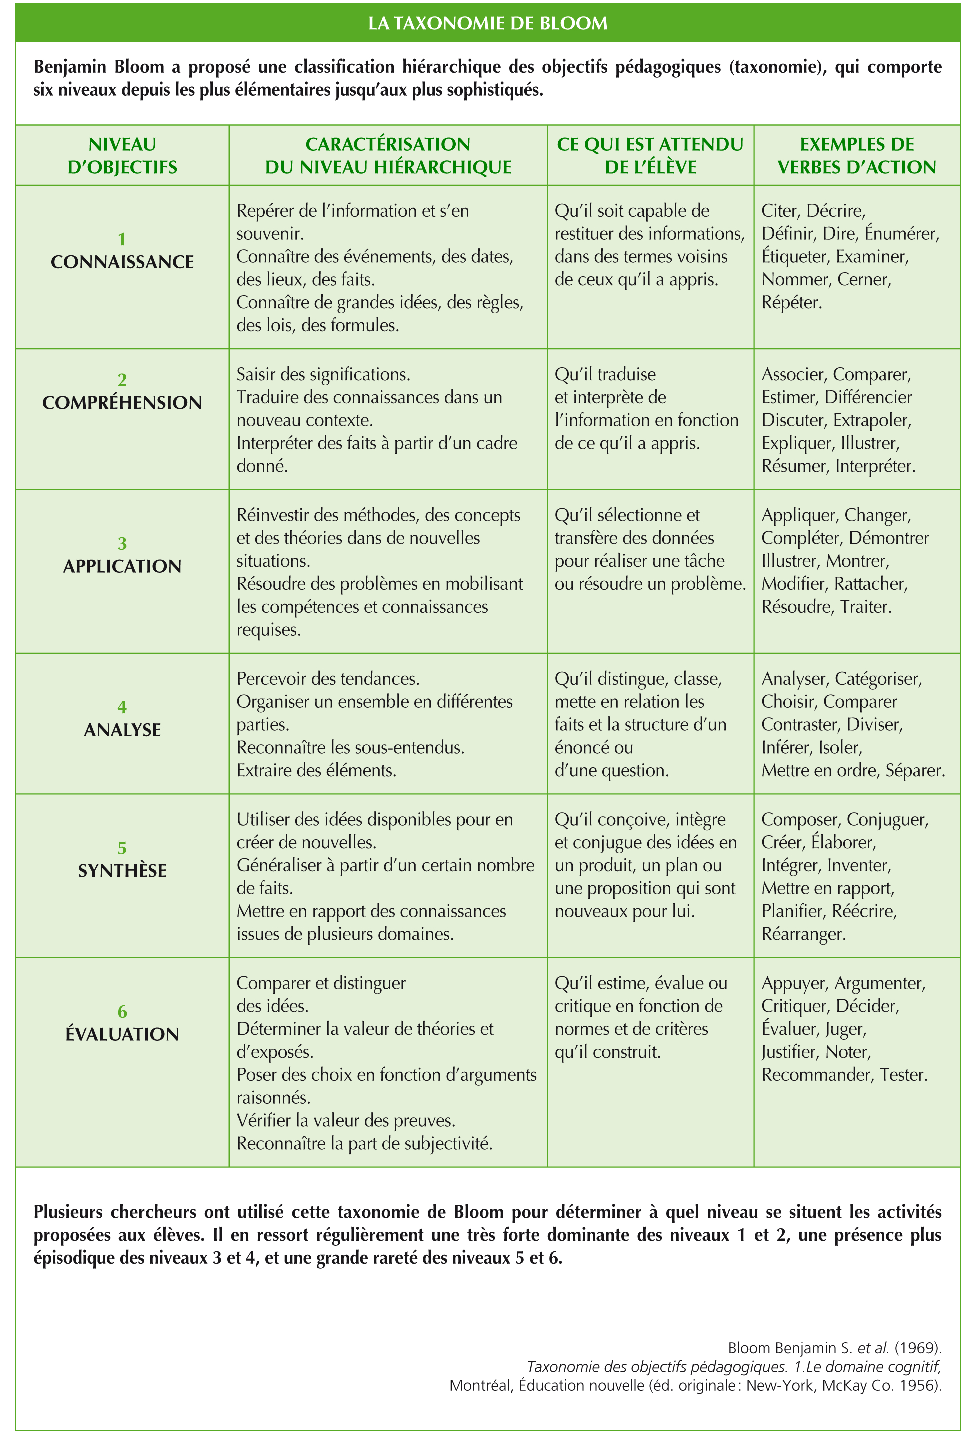
\includegraphics[width=0.9\textwidth]{bloom.pdf}
$$\fbox{\begin{minipage}{0.95\textwidth}\em
Dans toutes les disciplines, le questionnement est au c\oe ur de l'activité pédagogique. 
\emph{[\ldots]}

Il y aurait pourtant lieu de s'interroger sur la pratique qui consiste à interroger de but 
en blanc ceux que l'on place devant des objets culturels qui leur sont précisément étrangers.
Que peuvent-ils dire d'autre que des banalités bienfaisantes ? 
L'animateur le sait, tout comme le professeur, mais il n'attend souvent du
procédé qu'une occasion pour embrayer ses propres réponses, en faisant mine 
de les inscrire dans le fil de celles des élèves, par continuité
ou par contraste. Il oublie ainsi que l'on voit moins avec ses yeux qu'avec ses 
neurones, et qu'il n'est pas d'observation possible en l'absence de cadres interprétatifs. 
Le propre de l'expert c'est de disposer d'outils conceptuels lui
permettant de voir autre chose, et autrement que le commun des mortels. 
Ne dit-on pas que toute observation renseigne sur l'observateur ?
\emph{[\ldots]}

Examinons d'abord plus précisément les questions orales, qui montrent une curieuse
inversion par rapport aux formes quotidiennes du questionnement, en famille ou entre amis.
Dans ce cas, n'importe quelle réponse fait souvent l'affaire, et l'absence même de réponse
est fréquente, l'essentiel étant de pouvoir développer un échange de points de vue. Ou
alors, on pose une question à un plus expert que soi pour combler une ignorance, résoudre
un problème ou lever un doute. 
À l'école, au contraire, c'est le professeur qui interroge ceux qui, à l'évidence, 
en savent moins que lui ! Les élèves comprennent vite cette bizarrerie de la
« forme scolaire » et réalisent que le professeur, lui, ne cherche pas à s'informer 
mais à tester la classe. Dès la première question posée, flotte ainsi un parfum d'évaluation
informelle, avec ce qu'elle implique de violence symbolique. 
Contrairement au didactique familial, le propre du didactique scolaire c'est de 
travailler des questions ayant déjà des réponses, les élèves sachant parfaitement 
que le professeur les connaît. Du coup, ils cherchent à s'y adapter en inférant la 
réponse souhaitée, et ils répondent ainsi davantage au professeur pour satisfaire ses 
attentes qu'aux questions posées en vue de résoudre une énigme. 
Une analyse quantitative de séquences didactiques fait de
surcroît apparaître que le nombre de questions oralement posées est très élevé, 
ce qui renforce la nécessité pour les élèves de répondre de façon
stratégique. C'est ainsi qu'on peut parler d'un véritable « métier d'élève »!
\emph{[\ldots]}

Le questionnement sur des documents ou sur des manuels pose d'autres problèmes. 
Il conviendrait d'abord de clarifier, pour les élèves, sur quel mode on attend 
d'eux qu'ils répondent.
Faute de savoir le repérer, il arrive qu'ils répondent de façon très élaborée\ldots 
alors qu'on cherche seulement à s'assurer de la bonne compréhension
du texte; et, inversement, qu'ils fournissent une réponse qui reprend les termes du document\ldots
alors qu'on attend d'eux, cette fois, une mise en rapport de différents éléments pour 
développer une analyse critique. Pour le dire autrement, ils ne savent pas quel est le 
niveau d'objectif visé, tel que les a distingués Bloom : est-ce que cela
relève de la connaissance de faits particuliers, de la compréhension d'informations, 
de l'application d'une règle fournie, de l'analyse ou de la synthèse, voire d'une production critique qui combine la maîtrise objective des données avec un point de
vue personnel. 
Les élèves seraient grandement aidés si on leur précisait ainsi l'enjeu du 
questionnement (repérer une ou des informations contenues dans le texte, 
extraire du texte la ou les informations qui contiennent la réponse, mettre
en relation différents documents, interpréter le document à partir de cadres théoriques extérieurs, proposer une analyse plus subjective\ldots).
\emph{[\ldots]}
\end{minipage}}$$

%\textsc{Benjamin Bloom} a proposé une classification hiérarchique des objectifs pédagogiques 
%qui comporte 6 niveaux : connaissance, compréhension, application, analyse, 
%synthèse et évaluation. Cette taxonomie est résumée dans le tableau ci-dessous.
$$\begin{tabular}{|rl|p{3.5cm}|p{3.5cm}|p{3.5cm}|}
\hline
\multicolumn{5}{|c|}{\textsc{Taxonomie de Bloom}}\\
\multicolumn{5}{|c|}{\footnotesize Bloom B.S. et al., \emph{Taxonomy of educational objectives. Handbook I: the cognitive domain}, 1956}\\
\hline
\multicolumn{2}{|l|}{\textbf{Niveaux}} & \textbf{Caractéristiques} & \textbf{Capacités} & \textbf{Actions}\\
\hline
1. & connaissance 	& \footnotesize Repérer de l'information et s'en souvenir.
					  Connaître des événements, des dates, des lieux, des faits.
					  Connaître de grandes idées, des règles, des lois, des formules.
					& \footnotesize Etre capable de restituer des informations dans des termes voisins 
					  de ceux que l'on a appris.
					& \footnotesize citer, décrire, définir, dire, énumérer, étiqueter, examiner, 
					  nommer, cerner, répéter \\
\hline
2. & compréhension 	& \footnotesize Saisir des significa\-tions.
					  Traduire des con\-nais\-san\-ces dans un nouveau contexte.
					  Interpréter des faits à partir d'un cadre donné.
					& \footnotesize Etre capable de traduire et d'interpréter de l'information en fonction
					  de ce que l'on a appris.
					& \footnotesize associer, comparer, estimer, différentier, discuter, extrapoler, 
					  expliquer, illustrer, résumer, interpréter \\
\hline
3. & application 	& \footnotesize Réinvestir des méthodes, des concepts et des théories 
					  dans de nouvelles situations.
					  Résoudre des problèmes en mobilisant les compétences et connaissances
					  requises.
					& \footnotesize Etre capable de sélectionner et transférer des données pour 
					  réaliser une tâche ou résoudre un problème.
					& \footnotesize appliquer, changer, compléter, démontrer, illustrer, montrer,
					  modifier, rattacher, résoudre, traiter\\
\hline
4. & analyse 		& \footnotesize Percevoir des tendances.
					  Organiser un ensemble en différentes parties.
					  Reconnaître les sous-entendus.
					  Extraire des éléments.
					& \footnotesize Etre capable de distinguer, classer, mettre en relation les faits 
					  ou la structure d'un énoncé ou d'une question.
					& \footnotesize analyser, catégoriser, choisir, comparer, contraster, diviser,
					  inférer, isoler, ordonner, séparer \\
\hline
5. & synthèse 		& \footnotesize Utiliser des idées disponibles pour en créer de nouvelles.
					  Généraliser à partir d'un certain nombre de faits.
					  Mettre en rapport des connaissances issues de plusieurs domaines.
					& \footnotesize Etre capable de concevoir, intégrer et conjuguer des idées en un nouveau
					  produit, un nouveau plan ou une nouvelle proposition.
					& \footnotesize composer, conjuguer, créer, élaborer, intégrer, inventer, mettre en
					  rapport, planifier, réécrire, réarranger\\
\hline
6. & évaluation 	& \footnotesize Comparer et distinguer des idées.
					  Déterminer la valeur de théories et d'exposés.
					  Poser des choix en fonction d'arguments raisonnés.
					  Vérifier la valeur des preuves.
					  Reconnaître la part de subjectivité.
					& \footnotesize Etre capable d'estimer, d'évaluer ou de critiquer en
					  fonction de normes et de critères construits.
					& \footnotesize appuyer, argumenter, critiquer, décider, évaluer, juger,
					  justifier, noter, recommander, tester\\
\hline
\end{tabular}$$

$$\fbox{\begin{minipage}{0.95\textwidth}\em
Plus fondamentalement, le questionnement d'apprentissage devrait être distinct du
questionnement d'évaluation. Alors que le second vient souvent recouvrir le premier de
façon anticipée, comme si apprendre consistait à s'entraîner aux épreuves de contrôle\ldots 
En réalité, leur logique n'est pas la même. 
Contrairement au questionnement évaluatif, le questionnement d'apprentissage devrait 
s'intéresser davantage aux réponses incorrectes qu'aux réponses correctes, 
puisqu'il s'agit d'introduire les élèves à maîtriser des distinctions qu'ils 
sont en train d'apprendre. Toutes les réponses devraient être exploitées, analysées, 
comparées, puisqu'il s'agit de faire apprendre ! Surtout lorsqu'elles contiennent des 
erreurs « intéressantes » parce que régulières ou significatives. 
\emph{[\ldots]}

Les problèmes complexes posés par le questionnement pédagogique paraissent dus,
pour une large part, à la prééminence actuelle des méthodes inductives. 
On répète sur le mode de l'évidence que les notions doivent
toujours être introduites à partir d'exemples et d'activités concrètes, 
pour ne se dévoiler progressivement en tant que telles qu'au terme
du scénario. Le questionnement joue un rôle essentiel dans cet artifice, 
puisqu'il s'agit de faire dire par les élèves ce que précisément
ils ignorent, en évitant de l'imposer de façon dogmatique. 
On admettra que c'est là un principe préférable à celui d'un cours magistral
indigeste, mais il n'y a pas de raison que cela devienne une nouvelle « pensée unique » 
en pédagogie. En fait, il faut distinguer l'induction logique de l'induction pédagogique.

Sur le plan de la logique l'induction est une forme de raisonnement qui
vise à dégager une loi à partir de cas particuliers, à dépasser les exemples au 
profit d'un concept. En fait, elle n'est jamais épistémologiquement
valide, car elle comporte toujours le risque qu'un contre-exemple imprévu 
vienne contredire la généralisation. Le seul mode de raisonnement
rigoureux est la déduction, mais celle-ci ne produit rien de neuf, 
puisque tout est déjà inscrit dans les prémisses du syllogisme. 
L'induction court donc toujours le risque de la réfutation, 
mais elle est essentielle dans le progrès de la connaissance. 
Elle est à la base du raisonnement expérimental, en
permettant l'élaboration d'hypothèses plausibles.

Sur le plan pédagogique, l'induction est un procédé d'enseignement
partant d'exemples et d'expériences pratiques, et qui s'appuie sur eux 
pour introduire de façon intuitive une règle, une loi, un théorème.
Cette induction, actuellement préconisée dans de nombreuses disciplines, 
se démarque des pratiques traditionnelles qui commençaient par
énoncer la règle avant de proposer des exercices d'application. 
La question n'est pas ici celle de la validité logique, mais celle 
d'une compréhension qui serait plus progressive et naturelle.
Cette induction pédagogique est attrayante parce qu'elle semble plus concrète, 
plus proche des faits observables, mais le passage de l'exemple à la
notion rappelle souvent la prestidigitation, comme le lapin qui sort du chapeau. 
Elle est souvent illusoire, car seul l'enseignant voit dans l'exemple
le prototype d'une règle à venir, tandis que l'élève reste souvent scotché à l'exemple. 
Elle n'est donc pas sans vertu, mais il n'y a guère de raisons d'en
faire le « régime » unique du moteur de la classe.

Outre que cela allonge considérablement les séquences, il vaut sans doute mieux 
différencier les moments où l'on raisonne de façon « ascendante » (de l'exemple au concept) 
et ceux où l'on raisonne de façon « descendante » (du concept à l'exemple). 
Quoi qu'on fasse, il faut bien changer de registre à un moment ou un
autre, pour dégager la « pépite » conceptuelle de sa « gangue » d'exercices à 
répétition. 

\begin{flushright}
\textsc{Jean-Pierre Astolfi}, \emph{Le questionnement pédagogique}, \\
Economie et management, 128\char`\:68-73, juin 2008
\end{flushright}
\end{minipage}}$$

\newpage
%Lors d'un cours, il est assez fréquent qu'un enseignant réponde à des questions 
%que ses élèves ne se sont jamais posées.
Pour reprendre la terminologie de \textsc{Jean-Pierre Astolfi} dans l'encadré ci-dessus,
ce document est  conçu de façon plutôt «~ascendante~» (de l'exemple au concept) et se veut 
complémentaire des notes de cours \cite{cours} qui, elles, sont conçues plutôt classiquement
de façon «~descendante~» (du concept à l'exemple).

Nous introduisons donc ici une dizaine de questionnements qui couvrent
l'ensemble des notions abordées lors du cours d'informatique S1 de l'\enib.
Chaque questionnement concerne un point particulier du cours; il
est structuré en 5 parties de la manière suivante :
\begin{enumerate}
\item Exemple : dans cette partie, des questions « simples » sont posées 
	sur un problème «~connu~» de la «~vie courante~» afin d'introduire 
	le concept informatique sous-jacent. On y trouvera des
	exemples tels qu'
		aller au restaurant (section \ref{sec:algo}),
		ranger un meuble à tiroirs (\ref{sec:affectation}),
		analyser les sorties d'un circuit logique (\ref{sec:booleens}),
		compter avec \textsc{Bobby Lapointe} en base «~bibi~» (\ref{sec:codage}),
		déterminer sa mention au bac (\ref{sec:tests}),
		planter un clou (\ref{sec:boucles}),
		ranger des rondins de bois (\ref{sec:boucles-imbriquees}),
		cuisiner un quatre-quarts aux pépites de chocolat (\ref{sec:specification}),
		jouer aux tours de Hanoï  (\ref{sec:recursivite}) ou encore
		trier un jeu de cartes (\ref{sec:sequences}).
		
		Cette partie est principalement traitée par les étudiants eux-mêmes, individuellement ou 
		en groupe.
		
\item Généralisation : dans cette partie, les concepts informatiques sous-jacents
	sont présentés et introduits à l'aide de questions plus «~informatiques~».
	On y aborde les concepts 
	d'algorithmique (section \ref{sec:algo}),
	d'affectation (\ref{sec:affectation}),
	de calculs booléens (\ref{sec:booleens}),
	de codage des nombres (\ref{sec:codage}),
	de tests et d'alternatives (\ref{sec:tests}),
	de boucles (\ref{sec:boucles} et \ref{sec:boucles-imbriquees}),
	de spécification de fonction (\ref{sec:specification}),
	de récursivité (\ref{sec:recursivite}) ou encore
    de manipulation de séquences (\ref{sec:sequences}).

	En général, cette partie est traitée par l'enseignant.
	
\item Applications : des exemples « simples » d'application sont ensuite proposés.

	Le premier exemple est en général traité \emph{in extenso} par l'enseignant, les autres
	par les étudiants, en groupe ou individuellement.
	
\item Entraînement : cette partie est une préparation à l'évaluation qui a lieu
	en début de séance suivante. Les étudiants y travaillent chez eux entre les deux séances, 		
	individuellement ou en groupe.
	
	\begin{enumerate}
 	\item Enoncé : on présente ici le problème que l'on souhaite traiter tel que
 			le calcul en base «~Shadok~» (section \ref{sec:algo}),
 			le calcul de facteurs de conversion entre unités physiques (\ref{sec:affectation}),
 			l'établissement de la table de vérité d'une expression logique (\ref{sec:booleens}),
 			l'écriture d'un nombre réel selon la norme \textsc{Ieee} 754 (\ref{sec:codage}),
 			la détermination de la valeur d'une fonction continue et linéaire par morceaux (\ref{sec:tests}),
 			le calcul d'un développement limité selon une certaine précision (\ref{sec:boucles}),
 			le dessin d'un motif géométrique composé de polygones réguliers (\ref{sec:boucles-imbriquees}),
 			la spécification d'une fonction connue (un « grand classique » de la programmation) (\ref{sec:specification}),
 			le parcours d'un arbre binaire  (\ref{sec:recursivite}) ou encore
 			le tri d'un annuaire selon différents critères (\ref{sec:sequences}).
 			
 	\item Exemple : un exemple est traité en détail dans cette partie en insistant
 		sur la méthode pour arriver au résultat recherché et sur une ou des méthodes
 		de vérification du résultat obtenu.
 		
 	\item Questions : 24 questions de même difficulté sont proposées ici pour permettre 
 		à chaque étudiant de s'entraîner sur le problème à traiter.
 		
 		Le jour de l'évaluation, chaque étudiant traitera individuellement une des 24 questions
 		tirée au sort (une question différente par élève). Il sera demandé à chaque étudiant
 		de s'auto-évaluer selon 3 critères : la méthode pour arriver au résultat, 
 		le résultat lui-même et la vérification du résultat.
 		
 	\end{enumerate}
\item Révisions : Cette partie fait le lien entre ce document et les notes de cours
	\cite{cours,td}.
\end{enumerate}

\noindent
La conclusion «~tout en un~» reprend le premier exemple du document 
(exemple «~aller au restaurant~» de la section \ref{sec:algo}) et le traite intégralement 
d'un point de vue informatique afin de mettre en \oe uvre toutes les notions abordées 
dans le cours d'informatique S1 de l'\enib.
Finalement, la liste des 98 questions proposées dans ce document est donnée en annexe page \pageref{annexe:questions}.
